%! Author = jdubec
%! Date = 01/05/2026

\documentclass[11pt, a4paper]{article}

% ─── Packages ────────────────────────────────────────────────────────────────
\usepackage[utf8]{inputenc}
\usepackage[T1]{fontenc}
\usepackage[margin=2.5cm]{geometry}
\usepackage{graphicx}
\usepackage{hyperref}
\usepackage{booktabs}
\usepackage{float}
\usepackage{xcolor}
\usepackage{listings}
\hypersetup{colorlinks=true, linkcolor=black, citecolor=black, urlcolor=blue!70!black}

% ─── Code listing styles ────────────────────────────────────────────────────
\definecolor{codebg}{rgb}{0.97,0.97,0.97}
\definecolor{codekw}{rgb}{0.13,0.29,0.53}
\definecolor{codestr}{rgb}{0.55,0.10,0.10}
\definecolor{codecmt}{rgb}{0.30,0.55,0.30}

\lstset{
    basicstyle=\ttfamily\footnotesize,
    backgroundcolor=\color{codebg},
    breaklines=true,
    breakatwhitespace=true,
    breakindent=0pt,
    columns=fullflexible,
    keepspaces=true,
    frame=single,
    numbers=left,
    numberstyle=\tiny\color{gray},
    xleftmargin=1.2em,
    framexleftmargin=0.8em,
    showstringspaces=false,
    captionpos=b,
    postbreak=\mbox{\textcolor{gray}{$\hookrightarrow$}\space}
}

% ─── Bibliography ────────────────────────────────────────────────────────────
\usepackage[style=numeric, backend=bibtex]{biblatex}
\addbibresource{references.bib}

% ─── Line-breaking tolerance for long ttfamily tokens ───────────────────────
\sloppy
\setlength{\emergencystretch}{3em}

% ─── Language ────────────────────────────────────────────────────────────────
% Slovak language pack
\usepackage[slovak,shorthands=off]{babel}

\newcommand{\LabelProtocol}{Protokol k zadaniu}
\newcommand{\LabelCourse}{Databázové technológie}
\newcommand{\LabelCode}{DBS}
\newcommand{\LabelUniversity}{Slovenská technická univerzita v~Bratislave}
\newcommand{\LabelFaculty}{Fakulta informatiky a~informačných technológií}
\newcommand{\LabelAssignment}{Zadanie}
\newcommand{\LabelStudent}{Študent}
\newcommand{\LabelGroup}{Študijná skupina}
\newcommand{\LabelInstructor}{Cvičiaci}
\newcommand{\LabelDate}{Dátum}
\newcommand{\LabelYear}{Akademický rok}
\newcommand{\LabelContents}{Obsah}

% ─── Detaily študenta ────────────────────────────────────────────────────────
\newcommand{\StudentName}{Peter Mezei, David Blanko}
\newcommand{\StudyGroup}{Utorok 11:00}
\newcommand{\Instructor}{Emma Macháčová}
\newcommand{\AssignmentNumber}{3}
\newcommand{\AssignmentTitle}{Implementácia fyzického modelu a procesov - Správa kina}
\newcommand{\AcademicYear}{2025/2026}

\begin{document}

% ─── Titulná stránka ─────────────────────────────────────────────────────────
\begin{titlepage}
    \centering

    
\includegraphics[width=0.3\textwidth]{../assets/logo}

    \vspace{0.3cm}
    {\large \LabelUniversity}\\[2pt]
    {\large \LabelFaculty}

    \vspace{2.5cm}
    {\Huge\bfseries \LabelProtocol}

    \vspace{0.6cm}
    {\LARGE \LabelCode{} --- \LabelCourse}

    \vspace{0.4cm}
    {\Large \LabelAssignment{} \AssignmentNumber: \AssignmentTitle}

    \vfill

    \begin{tabular}{r l}
        \textbf{\LabelStudent:}    & \StudentName  \\[4pt]
        \textbf{\LabelGroup:}      & \StudyGroup   \\[4pt]
        \textbf{\LabelInstructor:} & \Instructor   \\[4pt]
        \textbf{\LabelYear:}       & \AcademicYear \\[4pt]
        \textbf{\LabelDate:}       & \today        \\
    \end{tabular}

    \vspace{1.5cm}
\end{titlepage}

% ─── Obsah ───────────────────────────────────────────────────────────────────
\renewcommand{\contentsname}{\LabelContents}
\tableofcontents
\newpage

% =============================================================================
\section{Zmeny oproti Zadaniu 1}
\label{sec:zmeny}

V tejto kapitole sumarizujeme úpravy fyzického modelu, ktoré sme spravili pri
implementácii v PostgreSQL oproti pôvodnému návrhu zo Zadania 1.

\begin{itemize}
    \item \textbf{Atribút \texttt{cena} presunutý z \texttt{listok}
    na \texttt{premietania}.} Pôvodne mal každý lístok vlastnú cenu,
    no v praxi sa cena tvorí na úrovni premietania (čas slotu, deň v týždni,
    typ sály) a všetky lístky daného premietania zdieľajú tú istú sumu.
    Tržba sa preto počíta ako \texttt{COUNT(listky)} $\times$
    \texttt{premietania.cena}.

    \item \textbf{Žáner, typ úväzku a typ úlohy implementované ako lookup
    tabuľky} (\texttt{zanre}, \texttt{typy\_uvazku}, \texttt{typy\_uloh}).
    Z pôvodného návrhu, kde to boli reťazcové atribúty, sme prešli na
    referenčnú integritu cez FK -- pridanie nového žánru / typu nevyžaduje
    schémovú zmenu (na rozdiel od ENUM-u).

    \item \textbf{Typ premietania zostal ako ENUM} (\texttt{'2D','3D'}) --
    množina je stabilná a nemení sa.

    \item \textbf{Pluralizácia názvov tabuliek} (\texttt{film}
    $\rightarrow$ \texttt{filmy}, \texttt{kinosala}
    $\rightarrow$ \texttt{kinosaly} atď.) -- štandardná SQL konvencia,
    odstraňuje konflikt s rezervovanými slovami.

    \item \textbf{Časové stĺpce: \texttt{DATETIME} $\rightarrow$
    \texttt{TIMESTAMP}.} PostgreSQL nemá typ \texttt{DATETIME},
    \texttt{TIMESTAMP (without time zone)} je priamy ekvivalent.

\end{itemize}

\begin{figure}[H]
    \centering
    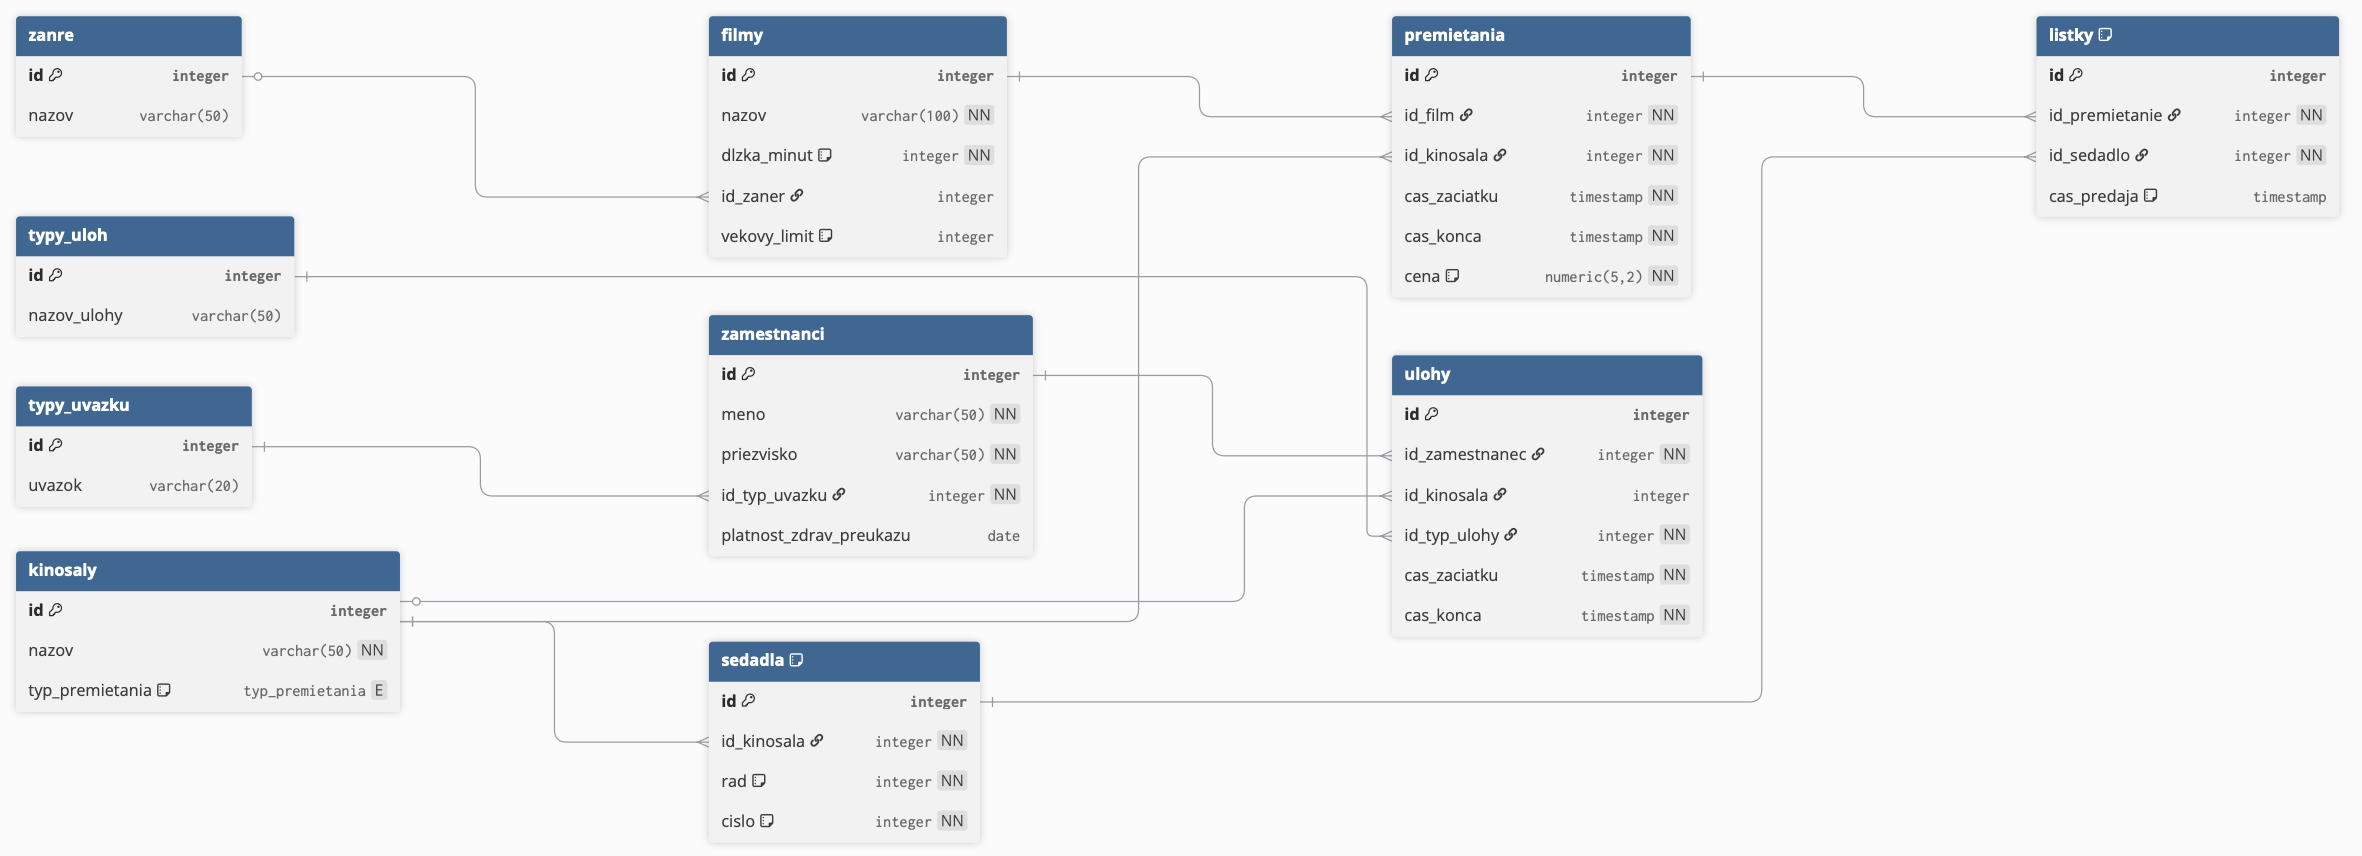
\includegraphics[width=\textwidth]{../../diagram}
    \caption{Aktualizovaný fyzický model po implementačných úpravách
             (10 tabuliek vrátane lookupov, ENUM \texttt{typ\_premietania},
             pluralizované názvy, \texttt{cena} na \texttt{premietania}).}
    \label{fig:relacny_model_v2}
\end{figure}

% =============================================================================
\newpage
\section{Fyzický model -- implementácia}
\label{sec:fyzicky_model}

Fyzický model je implementovaný v skripte \texttt{schema.sql} pre PostgreSQL
a obsahuje všetky tabuľky, integritné obmedzenia, ENUM typ a lookup tabuľky.

\subsection{Zoznam tabuliek}

\begin{table}[H]
    \centering
    \begin{tabular}{l p{9.5cm}}
        \toprule
        \textbf{Tabuľka} & \textbf{Stručný popis} \\
        \midrule
        \texttt{zanre}        & Lookup -- žánre filmov. \\
        \texttt{typy\_uvazku} & Lookup -- typy pracovného úväzku. \\
        \texttt{typy\_uloh}   & Lookup -- typy pracovných úloh. \\
        \texttt{filmy}        & Centrálny katalóg filmových titulov. \\
        \texttt{kinosaly}     & Fyzické miestnosti, v ktorých sa premieta. \\
        \texttt{sedadla}      & Konkrétne miesta v kinosále (rad, číslo). \\
        \texttt{premietania}  & Spojenie filmu, kinosály, časového slotu a ceny. \\
        \texttt{listky}       & Predaný lístok na konkrétne sedadlo a premietanie. \\
        \texttt{zamestnanci}  & Personálna evidencia. \\
        \texttt{ulohy}        & Pracovná úloha pridelená zamestnancovi v čase. \\
        \bottomrule
    \end{tabular}
    \caption{Prehľad tabuliek fyzického modelu.}
\end{table}

\subsection{Zaujímavé integritné obmedzenia}

\begin{itemize}
    \item \texttt{UNIQUE(id\_premietanie, id\_sedadlo)} v tabuľke
    \texttt{listky} -- na databázovej úrovni vynucuje biznis pravidlo č. 1
    (jedno sedadlo nemôže byť predané dvakrát na to isté premietanie).

    \item \texttt{UNIQUE(id\_kinosala, rad, cislo)} v tabuľke \texttt{sedadla}
    -- garantuje, že v rámci jednej kinosály neexistujú dve sedadlá
    s rovnakými súradnicami.

    \item \texttt{CHECK (dlzka\_minut > 0)} v tabuľke \texttt{filmy} --
    nuly a záporné dĺžky sú nezmysel.

    \item \texttt{CHECK (rad > 0)}, \texttt{CHECK (cislo > 0)} v tabuľke
    \texttt{sedadla} -- súradnice sedadla začínajú od 1.

    \item \texttt{CHECK (cena > 0)} v tabuľke \texttt{premietania} --
    cena lístka musí byť kladná.

    \item ENUM typ \texttt{typ\_premietania} (\texttt{'2D','3D'}) zužuje
    množinu povolených hodnôt už na úrovni typu.

    \item Lookup tabuľky (\texttt{zanre}, \texttt{typy\_uvazku},
    \texttt{typy\_uloh}) v kombinácii s FK obmedzeniami zaručujú, že
    žáner / typ úväzku / typ úlohy je vždy z definovanej množiny --
    a zároveň ostáva model rozšíriteľný bez zmeny schémy.
\end{itemize}

\subsection{Stratégie ON DELETE}

\begin{itemize}
    \item \texttt{kinosaly} $\rightarrow$ \texttt{sedadla}: \texttt{CASCADE}
    -- so zánikom sály zanikajú aj jej sedadlá (sedadlo nemá zmysel mimo sály).
    \item \texttt{filmy} $\rightarrow$ \texttt{premietania}: \texttt{RESTRICT}
    -- zabráni omylu vymazať film, na ktorý je naplánované premietanie.
    \item \texttt{kinosaly} $\rightarrow$ \texttt{premietania}: \texttt{RESTRICT}
    -- nemožno odstrániť sálu s naplánovaným programom.
    \item \texttt{premietania}, \texttt{sedadla} $\rightarrow$ \texttt{listky}:
    \texttt{RESTRICT} -- lístok je transakčný/finančný záznam, nesmie
    zmiznúť tichým mazaním.
    \item \texttt{zamestnanci} $\rightarrow$ \texttt{ulohy}: \texttt{CASCADE}
    -- pri výmaze zamestnanca (napr. GDPR) miznú aj jeho úlohy.
    \item \texttt{kinosaly} $\rightarrow$ \texttt{ulohy}: \texttt{CASCADE} --
    pri zániku sály miznú aj k nej viazané prevádzkové úlohy.
\end{itemize}

\subsection{Ukážka DDL}

\begin{lstlisting}[caption={Príklad definície tabuliek premietania a listky}]
CREATE TABLE premietania (
    id            SERIAL PRIMARY KEY,
    id_film       INT NOT NULL,
    id_kinosala   INT NOT NULL,
    cas_zaciatku  TIMESTAMP NOT NULL,
    cas_konca     TIMESTAMP NOT NULL,
    cena          NUMERIC(5, 2) NOT NULL CHECK (cena > 0),
    FOREIGN KEY (id_film)     REFERENCES filmy (id)     ON DELETE RESTRICT,
    FOREIGN KEY (id_kinosala) REFERENCES kinosaly (id)  ON DELETE RESTRICT
);

CREATE TABLE listky (
    id              SERIAL PRIMARY KEY,
    id_premietanie  INT NOT NULL,
    id_sedadlo      INT NOT NULL,
    cas_predaja     TIMESTAMP DEFAULT CURRENT_TIMESTAMP,
    FOREIGN KEY (id_premietanie) REFERENCES premietania (id) ON DELETE RESTRICT,
    FOREIGN KEY (id_sedadlo)     REFERENCES sedadla (id)     ON DELETE RESTRICT,
    UNIQUE (id_premietanie, id_sedadlo)
);
\end{lstlisting}

% =============================================================================
\newpage
\section{Seed dáta}
\label{sec:seed}

\subsection{Spôsob generovania}

Dáta generuje skript \texttt{seed/main.py} (Python 3 + \texttt{psycopg2}).
Skript je deterministický (\texttt{RNG\_SEED = 42}), na začiatku
\texttt{TRUNCATE \ldots RESTART IDENTITY CASCADE} všetky tabuľky a používa
\texttt{psycopg2.extras.\allowbreak execute\_values} pre rýchly batch insert.
Po vložení dát beží sada SQL kontrol (\texttt{validate\_generated\_data}),
ktorá v jednej transakcii overí 6 biznis pravidiel; ak ktorékoľvek zlyhá,
skript transakciu rollbackne.

\subsection{Počty záznamov}

\begin{table}[H]
    \centering
    \begin{tabular}{l r}
        \toprule
        \textbf{Tabuľka} & \textbf{Počet záznamov} \\
        \midrule
        zanre         & 10 \\
        typy\_uvazku  & 3 \\
        typy\_uloh    & 6 \\
        filmy         & 30 \\
        kinosaly      & 8 \\
        sedadla       & $\sim$1\,200 \\
        premietania   & $\sim$3\,500 \\
        zamestnanci   & 40 \\
        ulohy         & 120 \\
        listky        & $\sim$257\,000 \\
        \midrule
        \textbf{Spolu} & \textbf{$\sim$263\,000} \\
        \bottomrule
    \end{tabular}
    \caption{Počty záznamov po naplnení databázy (deterministický seed 42).}
\end{table}

\subsection{Zvolená distribúcia}

\begin{itemize}
    \item \textbf{Filmy:} 30 generovaných titulov, dĺžka 85--175 min,
    vekové limity vyvážené (najčastejšie 0/12/15/18).
    \item \textbf{Kinosály:} 8 sál (5 štandardných, 1 VIP, 1 rodinná, IMAX) --
    zmes 2D a 3D priestorov rôznej kapacity (70--240 sedadiel).
    \item \textbf{Premietania:} 90-dňový horizont (cca 30 dní v minulosti
    + 60 dní v budúcnosti, takže Proces 1 má reálne premietania na predaj),
    sloty 10:00--23:30, medzi predstaveniami 15--30 min na výmenu publika.
    Cena premietania závisí od dňa v týždni a hodiny (víkendová a večerná
    prirážka), čo zodpovedá reálnej tarifikácii.
    \item \textbf{Lístky:} obsadenosť závisí od slotu --
    ranné premietanie 15--45\,\%, popoludňajšie 30--70\,\%,
    večerné 45--95\,\%, víkend +5\,p.b. Tým vzniká výrazná variancia
    v tržbách medzi predstaveniami.
    \item \textbf{Zamestnanci:} 40 ľudí, 80\,\% s platným zdravotným preukazom.
    Úlohy s občerstvením (\texttt{Obsluha baru}) sa prideľujú výhradne
    zamestnancom s platným preukazom (biznis pravidlo č. 4).
\end{itemize}

\subsection{Konzistencia}

\begin{itemize}
    \item \textbf{Cudzie kľúče:} skript generuje záznamy v topologickom
    poradí (lookupy $\rightarrow$ \texttt{filmy}, \texttt{kinosaly},
    \texttt{sedadla} $\rightarrow$ \texttt{premietania}
    $\rightarrow$ \texttt{listky}, \texttt{ulohy}), takže FK referencie sú
    vždy platné.

    \item \textbf{Časová exkluzivita sály} (pravidlo č. 2) -- skript stavia
    rozpis sálu po sále chronologicky, vždy posunie začiatok ďalšieho slotu
    za koniec predošlého + 15--30 min nárazník. Žiadne dve premietania
    v jednej sále sa neprekrývajú.

    \item \textbf{Dostupnosť zamestnanca} (pravidlo č. 5) -- per-employee
    sa udržiava zoznam obsadených intervalov; nový pokus o pridanie úlohy
    sa zahodí pri preukázanom prekrytí (až do 250 pokusov, potom error).

    \item \textbf{Konzistencia sedadiel} (pravidlo č. 6) -- lístok sa
    generuje výhradne k sedadlu, ktoré patrí kinosále daného premietania
    (skript predtriedi sedadlá podľa \texttt{id\_kinosala}).

    \item \textbf{Validácia po seede} -- 6 nezávislých SQL kontrol
    (duplicitné lístky, prekrývajúce premietania, nadmerný predaj nad
    kapacitu, sedadlo mimo sály, občerstvenie bez preukazu, prekrývajúce
    úlohy zamestnanca). Pri zlyhaní transakcia rollbackne, skript skončí
    s chybou.
\end{itemize}

% =============================================================================
\newpage
\section{Proces 1 -- Transakčný predaj lístkov}
\label{sec:proces1}

\subsection{Popis a väzba na scenár}

Tento operačný proces zodpovedá \textbf{Scenáru 2} zo Zadania 1
(\emph{Transakčný predaj lístkov s alokáciou sedadiel}). Vstupom sú
\texttt{id\_premietanie} a \texttt{id\_sedadlo}. Výstupom je vytvorený
záznam v tabuľke \texttt{listky} -- za predpokladu, že sedadlo:
(a) patrí do tej istej kinosály, v ktorej beží dané premietanie,
(b) ešte nie je predané, a (c) premietanie sa ešte neskončilo.
Ak ktorákoľvek podmienka neplatí, \texttt{INSERT \ldots SELECT} vráti
0 riadkov a aplikácia ošetrí chybu.

Cena lístka sa neuvádza ako parameter -- je atribútom premietania.

Proces sa opiera o \texttt{UNIQUE(id\_premietanie, id\_sedadlo)} obmedzenie,
ktoré aj pri súčasnom prístupe garantuje, že jedno sedadlo nebude predané
dvakrát.

\subsection{Pomocný pohľad: dostupné sedadlá}

\begin{lstlisting}[caption={Pohľad: dostupné sedadlá pre dané (ešte neskončené) premietanie}]
CREATE OR REPLACE VIEW vw_dostupne_sedadla AS
SELECT  pr.id      AS id_premietanie,
        s.id       AS id_sedadlo,
        s.rad,
        s.cislo,
        k.nazov    AS sala,
        pr.cena
FROM    premietania pr
JOIN    kinosaly  k ON k.id = pr.id_kinosala
JOIN    sedadla   s ON s.id_kinosala = k.id
LEFT JOIN listky  l ON l.id_premietanie = pr.id
                   AND l.id_sedadlo     = s.id
WHERE   l.id IS NULL
  AND   pr.cas_konca > NOW();
\end{lstlisting}

\subsection{SQL implementácia (samotný predaj)}

\begin{lstlisting}[caption={Atomický INSERT lístka -- pure SQL, bez procedúr}]
INSERT INTO listky (id_premietanie, id_sedadlo)
SELECT  v.id_premietanie,
        v.id_sedadlo
FROM    vw_dostupne_sedadla v
WHERE   v.id_premietanie = :id_premietanie
  AND   v.id_sedadlo     = :id_sedadlo
RETURNING id, cas_predaja;
\end{lstlisting}

\subsection{Ukážka spustenia nad seed dátami}

\textbf{Vstup:} prvé budúce premietanie a sedadlo v rade 1, číslo 1.
Zachytené proti reálne naseednutej databáze.

\textbf{(1) Pre-flight -- voľné sedadlá pre dané premietanie:}
\begin{verbatim}
 id_premietanie | id_sedadlo | rad | cislo |  sala  | cena
----------------+------------+-----+-------+--------+------
            148 |          1 |   1 |     1 | SALA 1 | 8.21
            148 |          2 |   1 |     2 | SALA 1 | 8.21
            148 |          4 |   1 |     4 | SALA 1 | 8.21
            148 |          5 |   1 |     5 | SALA 1 | 8.21
            148 |          7 |   1 |     7 | SALA 1 | 8.21
\end{verbatim}

\textbf{(2) Vlastný predaj:}
\begin{verbatim}
   id   | id_premietanie | id_sedadlo |        cas_predaja
--------+----------------+------------+----------------------------
 257665 |            148 |          1 | 2026-05-02 11:25:37.515468
INSERT 0 1
\end{verbatim}

\textbf{(3) Zopakovanie tej istej operácie} -- \texttt{INSERT} vracia
0 riadkov, lebo sedadlo už nie je vo \texttt{vw\_dostupne\_sedadla}:
\begin{verbatim}
 id
----
(0 rows)
INSERT 0 0
\end{verbatim}

\textbf{Korektnosť:} idempotencia je preukázaná opakovaným spustením
toho istého dopytu -- prvý prebehne, druhý vráti prázdnu množinu bez
chyby. Pri konkurenčnom prístupe by namiesto toho zafungoval
\texttt{UNIQUE(id\_premietanie, id\_sedadlo)} a klient by dostal
``duplicate key value violates unique constraint'' (transakcia rollbackne).

\subsection{Indexy podporujúce tento proces}

\begin{itemize}
    \item \texttt{idx\_listky\_premietanie} na \texttt{listky(id\_premietanie)}
    -- urýchľuje \texttt{LEFT JOIN} v pohľade pri overovaní obsadenosti.
    \item \texttt{idx\_sedadla\_kinosala} na \texttt{sedadla(id\_kinosala)}
    -- urýchľuje vyhľadanie všetkých sedadiel pre danú sálu.
    \item Implicitný UNIQUE index nad \texttt{(id\_premietanie, id\_sedadlo)}
    je využitý pri kontrole duplicity a pri samotnom \texttt{INSERT}.
\end{itemize}

% =============================================================================
\newpage
\section{Proces 2 -- Štatistika predajnosti filmov}
\label{sec:proces2}

\subsection{Popis a väzba na scenár}

Analytický proces zodpovedá \textbf{Scenáru 4} zo Zadania 1
(\emph{Generovanie agregovaných štatistík predajnosti}). Vstupom je časový
interval (\texttt{:od}, \texttt{:do}); výstupom je tabuľka filmov zoradená
podľa tržby s informáciami: počet premietaní, počet predaných lístkov,
priemerná cena, tržba, obsadenosť (\,\%) a poradie v rebríčku.

\subsection{SQL implementácia}

Cena je atribútom premietania, takže tržbu počítame ako
\texttt{COUNT(listky)} $\times$ \texttt{premietania.cena} -- priemerná cena
predaného lístka môže byť rôzna pre rôzne premietania toho istého filmu
(víkendová a večerná prirážka).

\begin{lstlisting}[caption={Analytický dopyt: predajnosť filmov za zvolené obdobie}]
WITH kapacita_kinosaly AS (
    SELECT  k.id        AS id_kinosala,
            COUNT(s.id) AS kapacita
    FROM    kinosaly k
    JOIN    sedadla  s ON s.id_kinosala = k.id
    GROUP BY k.id
),
filtrovane_premietania AS (
    SELECT  p.id,
            p.id_film,
            p.cena,
            kk.kapacita
    FROM    premietania p
    JOIN    kapacita_kinosaly kk ON kk.id_kinosala = p.id_kinosala
    WHERE   p.cas_zaciatku >= :od
      AND   p.cas_zaciatku <  (:do::timestamp + INTERVAL '1 day')
),
predane_na_premietanie AS (
    SELECT  l.id_premietanie,
            COUNT(*) AS predane_listky
    FROM    listky l
    GROUP BY l.id_premietanie
),
predaj_film AS (
    SELECT  f.id                              AS id_film,
            f.nazov                           AS nazov_filmu,
            fp.id                             AS id_premietania,
            fp.cena                           AS cena_premietania,
            fp.kapacita                       AS kapacita,
            COALESCE(pnp.predane_listky, 0)   AS predane_listky
    FROM    filtrovane_premietania fp
    JOIN    filmy f                ON f.id  = fp.id_film
    LEFT JOIN predane_na_premietanie pnp
                                  ON pnp.id_premietanie = fp.id
)
SELECT
    nazov_filmu,
    COUNT(*)                                  AS pocet_premietani_s_predajom,
    SUM(predane_listky)                       AS predane_listky_spolu,
    ROUND(SUM(predane_listky * cena_premietania), 2) AS trzba_spolu_eur,
    ROUND(AVG(predane_listky), 2)             AS priemer_listkov_na_premietanie,
    ROUND(
        SUM(predane_listky * cena_premietania) /
        NULLIF(SUM(predane_listky), 0), 2
    )                                         AS priemerna_cena_predaneho_listka_eur,
    ROUND(
        100.0 * SUM(predane_listky) /
        NULLIF(SUM(kapacita), 0), 2
    )                                         AS obsadenost_pct,
    RANK() OVER (
        ORDER BY SUM(predane_listky * cena_premietania) DESC
    )                                         AS poradie_podla_trzby
FROM   predaj_film
GROUP BY nazov_filmu
ORDER BY trzba_spolu_eur DESC, predane_listky_spolu DESC;
\end{lstlisting}

\subsection{Ukážka spustenia nad seed dátami}

\textbf{Vstup:} \texttt{:od = '2026-04-01'}, \texttt{:do = '2026-04-30'}
(jeden mesiac).

\textbf{Výstup -- top 10 filmov podľa tržby:}
{\scriptsize
\begin{verbatim}
              nazov_filmu              | premietani | listkov | trzba_eur | prum_cena | obsadenost_pct | poradie
---------------------------------------+------------+---------+-----------+-----------+----------------+---------
 Zabudnuty Tieň: V hlavnej ulohe noc   |         48 |    4264 |  44157.17 |     10.36 |          56.80 |       1
 Ohnivy Horizont: Mimo pravidiel       |         42 |    3286 |  35185.73 |     10.71 |          52.58 |       2
 Skryty Misia                          |         45 |    3400 |  34617.30 |     10.18 |          50.11 |       3
 Zabudnuty Svetlo                      |         39 |    3138 |  34530.50 |     11.00 |          50.92 |       4
 Ohnivy Signal                         |         41 |    3099 |  33962.17 |     10.96 |          47.52 |       5
 Tichy Misia: Posledna kapitola        |         43 |    3215 |  33954.00 |     10.56 |          51.63 |       6
 Nocturny Lovec: V tieni pravdy        |         41 |    3397 |  33662.40 |      9.91 |          50.28 |       7
 Tichy Experiment: V hlavnej ulohe noc |         49 |    3321 |  33364.31 |     10.05 |          47.15 |       8
 Temny Hrad                            |         42 |    3083 |  32755.53 |     10.62 |          50.98 |       9
 Ohnivy Most                           |         42 |    3195 |  31821.09 |      9.96 |          50.22 |      10
\end{verbatim}
}

\textbf{Korektnosť overená dvomi spôsobmi:}
\begin{enumerate}
    \item Súčet stĺpca \texttt{trzba\_eur} naprieč všetkými filmami sa
    rovná kontrolnému dopytu:
\begin{lstlisting}
SELECT SUM(p.cena)
FROM   listky l
JOIN   premietania p ON p.id = l.id_premietanie
WHERE  p.cas_zaciatku BETWEEN :od AND :do;
\end{lstlisting}
    \item Stĺpec \texttt{prum\_cena} (priemerná cena predaného lístka pre
    daný film) má hodnoty v rozumnom rozsahu 9,91--11,00 EUR -- variancia
    odráža kombináciu víkendovej a večernej prirážky pri rôznych
    premietaniach toho istého filmu.
\end{enumerate}

\subsection{Indexy podporujúce tento proces}

\begin{itemize}
    \item \texttt{idx\_premietania\_interval\_film} na
    \texttt{premietania(cas\_zaciatku, id, id\_film)} -- kompozitný index pre
    range filter \texttt{cas\_zaciatku} a následný JOIN na film.
    \item \texttt{idx\_listky\_premietanie} na \texttt{listky(id\_premietanie)}
    -- urýchľuje \texttt{GROUP BY id\_premietanie} v CTE
    \texttt{predane\_na\_premietanie}.
    \item \texttt{idx\_filmy\_id\_nazov} na \texttt{filmy(id) INCLUDE (nazov)}
    -- covering index pre finálny JOIN -- vie čítať \texttt{nazov} priamo
    z indexu bez prístupu do haldy.
\end{itemize}

% =============================================================================
\newpage
\section{Výkonnosť a indexy}
\label{sec:vykonnost}

\subsection{Zoznam vytvorených indexov}

\begin{table}[H]
    \centering
    \begin{tabular}{l p{4.5cm} p{5cm}}
        \toprule
        \textbf{Názov indexu} & \textbf{Tabuľka(stĺpec)} & \textbf{Účel} \\
        \midrule
        idx\_listky\_premietanie         & listky(id\_premietanie)     & FK lookup pri JOIN v Procese 1 a agregácii v Procese 2 \\
        idx\_premietania\_interval\_film & premietania(cas\_zaciatku, id, id\_film) & Kompozitný index pre range filter \texttt{BETWEEN} a JOIN na film v Procese 2 \\
        idx\_filmy\_id\_nazov            & filmy(id) INCLUDE (nazov)   & Covering index pre čítanie názvu bez prístupu do haldy v Procese 2 \\
        idx\_sedadla\_kinosala           & sedadla(id\_kinosala)       & Mapa sedadiel pre danú sálu v Procese 1 \\
        \bottomrule
    \end{tabular}
    \caption{Súhrn indexov nad rámec PK/UNIQUE.}
\end{table}

\subsection{EXPLAIN (ANALYZE, BUFFERS) -- pred a po pridaní indexu}

\textbf{Dopyt:} top-10 najpredávanejších filmov za 8-mesačné obdobie
(Proces 2).

\textbf{Skutočne použitý dopyt:} top filmov za jeden konkrétny deň (24-h
okno). Zúžili sme okno z mesiaca na deň, aby filter bol dostatočne
selektívny -- pri 1-dňovom okne pripadá na obdobie 38 z 3\,489 premietaní
($\sim$1\,\%), takže index naozaj zmení plán.

\begin{lstlisting}[caption={Analytika za jeden deň, použitá pre EXPLAIN}]
EXPLAIN (ANALYZE, BUFFERS)
WITH filtrovane_premietania AS (
    SELECT p.id, p.id_film, p.cena
    FROM   premietania p
    WHERE  p.cas_zaciatku >= '2026-04-15'
      AND  p.cas_zaciatku <  '2026-04-16'
),
predane_na_premietanie AS (
    SELECT l.id_premietanie, COUNT(*) AS predane_listky
    FROM   listky l
    JOIN   filtrovane_premietania fp ON fp.id = l.id_premietanie
    GROUP  BY l.id_premietanie
)
SELECT f.nazov,
       SUM(pnp.predane_listky)            AS listkov,
       ROUND(SUM(pnp.predane_listky * fp.cena), 2) AS trzba_eur,
       RANK() OVER (ORDER BY SUM(pnp.predane_listky * fp.cena) DESC)
                                          AS poradie
FROM   filtrovane_premietania fp
JOIN   filmy f ON f.id = fp.id_film
LEFT  JOIN predane_na_premietanie pnp ON pnp.id_premietanie = fp.id
GROUP  BY f.nazov
ORDER  BY trzba_eur DESC
LIMIT  10;
\end{lstlisting}

\textbf{Pred pridaním indexov} (žiadne vlastné indexy, iba PK/UNIQUE):
\begin{lstlisting}[caption={Plán pred indexmi -- skrátené, kľúčové uzly}]
Limit  (cost=408.69..408.71 rows=10) (actual time=0.561..0.563)
  Buffers: shared hit=152
  ->  Seq Scan on premietania p
        Filter: (cas_zaciatku >= '2026-04-15' AND cas_zaciatku < '2026-04-16')
        Rows Removed by Filter: 3451
        Buffers: shared hit=30
  ->  Index Only Scan using listky_id_premietanie_id_sedadlo_key on listky l
        Index Cond: (id_premietanie = fp_1.id)
        Buffers: shared hit=118
Planning Time: 0.435 ms
Execution Time: 0.616 ms
\end{lstlisting}

\textbf{Po pridaní troch indexov} (\texttt{idx\_listky\_premietanie},
\texttt{idx\_premietania\_interval\_film}, \texttt{idx\_filmy\_id\_nazov}):
\begin{lstlisting}[caption={Plán po vytvorení indexov -- skrátené, kľúčové uzly}]
Limit  (cost=350.62..350.65 rows=10) (actual time=0.428..0.430)
  Buffers: shared hit=79 read=14
  ->  Bitmap Heap Scan on premietania p
        Recheck Cond: (cas_zaciatku >= '2026-04-15' AND cas_zaciatku < '2026-04-16')
        Heap Blocks: exact=8
        ->  Bitmap Index Scan on idx_premietania_interval_film
              Index Cond: (...same...)
              Buffers: shared read=3
  ->  Index Only Scan using idx_listky_premietanie on listky l
        Index Cond: (id_premietanie = fp_1.id)
        Buffers: shared hit=67 read=11
Planning Time: 0.564 ms
Execution Time: 0.494 ms
\end{lstlisting}

\textbf{Čo sa zmenilo:}

\begin{itemize}
    \item \texttt{Seq Scan on premietania} (filtruje 3\,451 z 3\,489
    riadkov) sa nahradil \texttt{Bitmap Index Scan on
    idx\_premietania\_interval\_film} -- index Recheck číta iba 8 heap
    blokov namiesto 30, pretože kvalifikujúce sa premietania sú
    lokalizované v zopár stránkach.

    \item Plánovač prepol z implicitného UNIQUE indexu
    \texttt{listky\_id\_premietanie\_id\_sedadlo\_key} (12 B kľúč) na
    užší \texttt{idx\_listky\_premietanie} (4 B kľúč) -- menší index
    znamená menej stránok pri Index Only Scan-e.

    \item \textbf{Buffers} klesli z \texttt{shared hit=152} na
    \texttt{shared hit=79 + read=14 = 93} ($\sim$39\,\% menej dotykov
    bufferov).

    \item \textbf{Execution Time} klesol z \,0,616\,ms na 0,494\,ms
    ($\sim$20\,\% zrýchlenie). Absolútne čísla sú malé, lebo sa dataset
    vojde do \texttt{shared\_buffers}; pri reálnom (väčšom) sklade
    by efekt indexu na \texttt{premietania} narastal lineárne s počtom
    riadkov.
\end{itemize}

\subsection{Dopyty, ktoré zostali pomalé}

\begin{itemize}
    \item \textbf{Plný analytický pohľad za celý mesiac alebo dlhšie}
    -- pri 30-dňovom okne ($\sim$1\,130 premietaní z 3\,489, teda
    32\,\% riadkov) plánovač naďalej preferuje \texttt{Seq Scan} aj
    v prítomnosti \texttt{idx\_premietania\_interval\_film}.
    Je to očakávané: keď filter necháva tretinu tabuľky, index lookup
    + heap fetch je drahší ako sekvenčné čítanie.
    Riešením by bol \texttt{MATERIALIZED VIEW} osviežovaný napríklad
    denne v noci.

    \item \textbf{Plná agregácia \texttt{listky}} pri Procese 2 nad
    veľkým rozsahom -- aj s indexom musí dopyt prečítať všetky lístky
    ($\sim$257\,k riadkov), keďže nemáme \texttt{WHERE} filter na
    \texttt{listky}. To by sa dalo optimalizovať partícionovaním
    \texttt{listky} podľa \texttt{cas\_predaja}.
\end{itemize}

% =============================================================================
\newpage
\section{Zhodnotenie}
\label{sec:zhodnotenie}

\begin{itemize}
    \item \textbf{Ktorá časť vás prekvapila -- seed, dopyty alebo indexy?
    Prečo?} \\
    TODO

    \item \textbf{Narazili ste pri implementácii na chybu v pôvodnom modeli?
    Ako ste ju opravili?} \\
    TODO

    \item \textbf{Ktoré biznis pravidlo bolo v SQL najťažšie vyjadriť a prečo?} \\
    TODO

    \item \textbf{Použili ste AI nástroje? Na čo presne, aký bol výstup
    a ako ste ho upravovali?} \\
    TODO
\end{itemize}

\printbibliography

\end{document}
